Together with the NASA \ac{PSP} launched in August 2018, the ESA \ac{SolO} mission ushers in a new era in solar and heliospheric physics. For the first time since the 1970s, these spacecraft will approach the Sun significantly closer than the orbit of Mercury --- \ac{PSP} has already set a new record with less than \SI{0.1}{\AU} solar distance at its most recent perihelion in September 2020. On the other hand, \ac{SolO}, which was launched in February 2020, will come very close to the Sun as well ($\sim\SI{0.28}{\AU}$), although it will stay far enough away to also allow for imaging observations through holes in its heatshield. In the extended mission phase, it is planned to incline the orbit of \ac{SolO} to also observe the poles of the Sun for the first time.

As part of the \ac{EPD} suite on \ac{SolO} \citep{RodriguezPacheco-2019-EPD}, the \acl{HET}\acused{HET} (\acs{HET}, \autoref{sec:solohet}) has been successfully commissioned and is providing some first measurements of high-energy charged particles. While a few \ac{SEP} events in the first 10 months of the mission did extend to the energies covered by \ac{HET} ($\gtrsim\SI{6}{\mega\electronvolt\per nuc}$ ions and $>\SI{450}{\kilo\electronvolt}$ electrons), \ac{HET} spent most of the time observing the \ac{GCR} background, as the Sun was very quiet during this time. As discussed in \autoref{sec:solohet}, \ac{HET} is also able to resolve short-term variations of \acp{GCR} with some of its data products. Consequently, some \acp{FD} could be measured, which were caused by \acp{CME} and \acp{CIR} that passed \ac{SolO} during its first orbit.

The first \ac{FD} seen at \ac{SolO} caused by a \ac{CME} on April 19, 2020 is especially interesting, as it is a multispacecraft event that was also observed near Earth one day later during a close longitudinal alignment and with a radial separation of \SI{0.2}{\AU}. Measurements of the \ac{FD} near Earth have been taken by neutron monitors as well as the \ac{CRaTER} onboard the \ac{LRO}. The \ac{CME} was also seen at the BepiColombo spacecraft that was still close to Earth at this time, and may also have hit Venus, though no observations at Venus are available due to the loss of contact with the Venus Express spacecraft since 2014. Furthermore, \acs{STEREO}-A was in a perfect position to provide a side view of the \ac{CME} with its remote sensing instruments. In the following publication, which was submitted to \textit{Astronomy \& Astrophysics} in November 2020, we describe the capabilities of \ac{HET}, present the \ac{FD} observed at \ac{SolO} and the corresponding observations near Earth, and investigate the radial evolution of the \ac{CME} by applying \acs{ForbMod} (see \autoref{sec:forbush}) to this event. Another study of the same event, focusing on the magnetic field observations, has also been submitted by Emma E. Davies of Imperial College London, and both will be published in the ``Solar Orbiter First Results'' special issue of \textit{A\&A} in 2021.

In the process of this study, a new implementation of the \ac{GCS} model \citep{Thernisien-2011-GCS} was developed. Details about this software can be found in \autoref{chp:GCS_Python}.

The following article is reproduced from \textcite{Forstner-2021-SolO} with permission from Astronomy \& Astrophysics, \copyright  ESO:\\

\noindent
\pubcite{Forstner-2021-SolO}
\hfill Own contribution: 80\%

\newpage
\newcounter{includepdfpageAATwentyOne}

\addtocounter{section}{1}
\setcounter{subsection}{1} 
\phantomsection
\addcontentsline{toc}{section}{\arabic{chapter}.\arabic{section} Radial Evolution of the April 2020 Stealth Coronal Mass Ejection between 0.8 and 1 AU: A Comparison of Forbush Decreases at Solar Orbiter and Earth (Publication A\&A 2021)}
%
\phantomsection
\addcontentsline{toc}{subsection}{\arabic{chapter}.\arabic{section}.\arabic{subsection} Introduction}
\label{sec:paper_forstner2021}
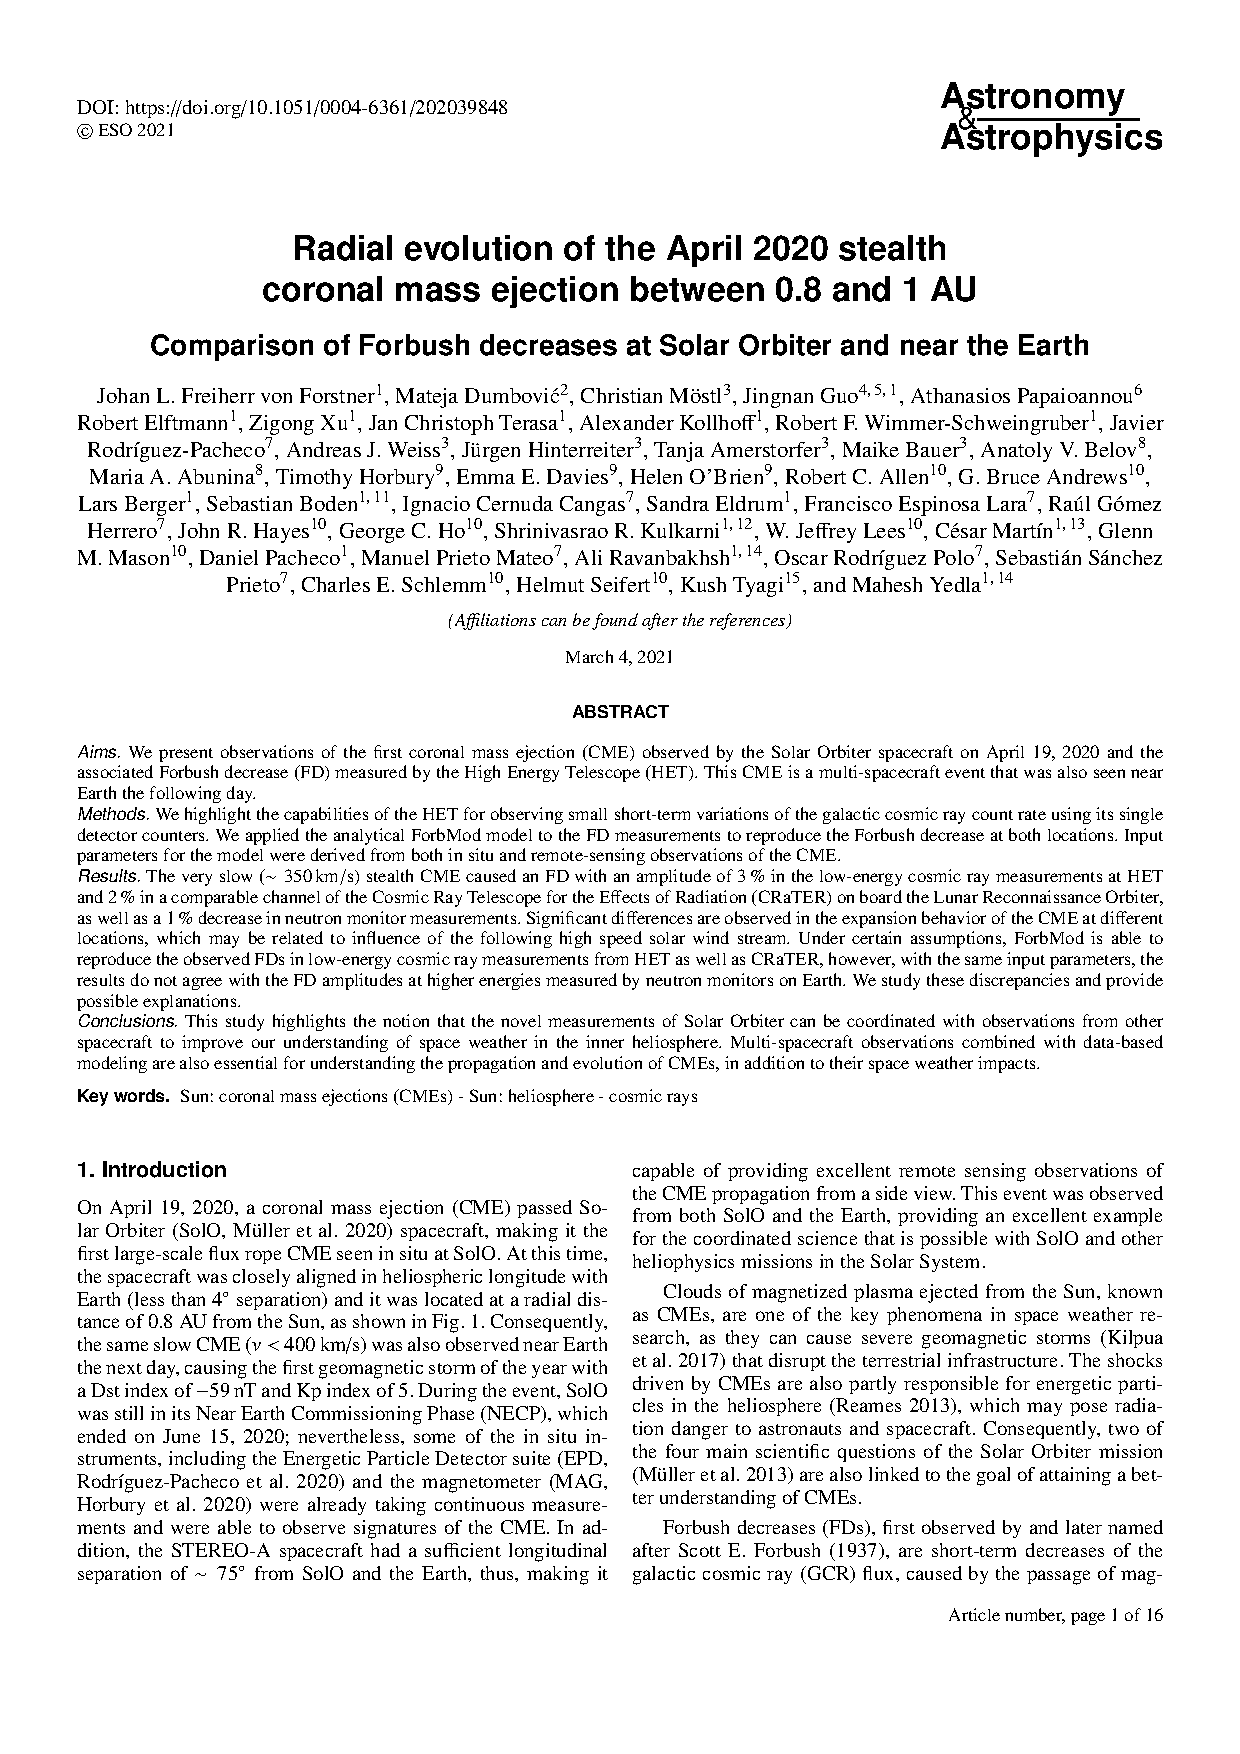
\includepdf[pages={1}, link, linkname=paper_forstner2021, scale=.95, pagecommand={\refstepcounter{includepdfpageAATwentyOne}\label{paper_forstner2021.\theincludepdfpageAATwentyOne}}]{publications/Forstner_et_al-2021-AandA.pdf}
%
\addtocounter{subsection}{1} 
\phantomsection
\addcontentsline{toc}{subsection}{\arabic{chapter}.\arabic{section}.\arabic{subsection} Data Sources}
\includepdf[pages={2-4}, link, linkname=paper_forstner2021, scale=.95, pagecommand={\refstepcounter{includepdfpageAATwentyOne}\label{paper_forstner2021.\theincludepdfpageAATwentyOne}}]{publications/Forstner_et_al-2021-AandA.pdf}
%
\addtocounter{subsection}{1} 
\phantomsection
\addcontentsline{toc}{subsection}{\arabic{chapter}.\arabic{section}.\arabic{subsection} Methods}
%
\addtocounter{subsection}{1} 
\phantomsection
\addcontentsline{toc}{subsection}{\arabic{chapter}.\arabic{section}.\arabic{subsection} Results}
\includepdf[pages={5-10}, link, linkname=paper_forstner2021, scale=.95, pagecommand={\refstepcounter{includepdfpageAATwentyOne}\label{paper_forstner2021.\theincludepdfpageAATwentyOne}}]{publications/Forstner_et_al-2021-AandA.pdf}
%
\addtocounter{subsection}{1} 
\phantomsection
\addcontentsline{toc}{subsection}{\arabic{chapter}.\arabic{section}.\arabic{subsection} Discussion and conclusions}
\includepdf[pages={11-13}, link, linkname=paper_forstner2021, scale=.95, pagecommand={\refstepcounter{includepdfpageAATwentyOne}\label{paper_forstner2021.\theincludepdfpageAATwentyOne}}]{publications/Forstner_et_al-2021-AandA.pdf}
%
\addtocounter{subsection}{1} 
\phantomsection
\addcontentsline{toc}{subsection}{\arabic{chapter}.\arabic{section}.\arabic{subsection} References}
\includepdf[pages={14-15}, link, linkname=paper_forstner2021, scale=.95, pagecommand={\refstepcounter{includepdfpageAATwentyOne}\label{paper_forstner2021.\theincludepdfpageAATwentyOne}}]{publications/Forstner_et_al-2021-AandA.pdf}
%